\label{chap:results}
\begin{table*}[]
\centering
\caption{Summary of results for \texttt{bmi\_refresh}, \texttt{static\_batch},
\texttt{partial\_refresh} and \texttt{precision\_strategy}}
\label{table.summary}
\resizebox{\textwidth}{!}{%
\begin{tabular}{|c|c|c|c|c|c|}
\hline
\textbf{Strategy} & \begin{tabular}[x]{@{}c@{}}
    \textbf{Avg. Recall}\\ \textbf{@($E_{norm}$=1)}
\end{tabular} & \begin{tabular}[x]{@{}c@{}}
\textbf{Avg. Recall}\\ \textbf{@($E_{norm}$=1.5)}
\end{tabular} & \begin{tabular}[x]{@{}c@{}}
\textbf{Avg. Recall}\\ \textbf{@($E_{norm}$=2)}
\end{tabular} & \begin{tabular}[x]{@{}c@{}}
\textbf{$E_{norm}$ for}\\ \textbf{75\% recall}
\end{tabular}&
\begin{tabular}[x]{@{}c@{}}
    \textbf{Running Time}\\ \textbf{(in min)}
\end{tabular} \\ \hline \hline
\texttt{bmi}& 0.715 & 0.827 & 0.905 & 1.128 & 0.22 \\ \hline \hline
\texttt{static(k=1)} & 0.750 & 0.865 & 0.926 & 1.021 & 49.29 \\ \hline
\texttt{static(k=100)} &  0.704 & 0.807 & 0.887 & 1.167 & 0.47 \\ \hline \hline
\texttt{partial(k=10,s=1000)} &  0.753 & 0.862 & 0.926 & 1.008 & 40.92 \\ \hline
\texttt{partial(k=100,s=500)} &  0.753 & 0.855 & 0.923 & 1.022 & 38.28 \\ \hline
\texttt{partial(k=100,s=1000)} &  0.754 & 0.856 & 0.922 & 1.013 & 39.57 \\ \hline
\texttt{partial(k=100,s=5000)} &  0.756 & 0.855 & 0.921 & 1.016 & 40.70 \\ \hline
\texttt{partial(k=500,s=1000)} &  0.700 & 0.785 & 0.815 & 1.324 & 38.63\\
\hline \hline
\texttt{precision(m=25,p=0.4)} &  0.698 & 0.849 & 0.915 & 1.129 & 35.68 \\ \hline
\texttt{precision(m=25,p=0.6)} &  0.735 & 0.859 & 0.923 & 1.059 & 40.20 \\ \hline
\texttt{precision(m=25,p=0.8)} &  0.750 & 0.862 & 0.926 & 1.024 & 44.64 \\ \hline
\texttt{precision(m=25,p=1.0)} &  0.752 & 0.865 & 0.926 & 1.014 & 47.41 \\
\hline
% recency\_weighting($w=1$,$it=1000$) &  0.704 & 0.798 & 0.875 & 1.243 & 11.75 \\ \hline
% recency\_weighting($w=2$,$it=1000$) &  0.705 & 0.806 & 0.884 & 1.219 & 11.66 \\ \hline
% recency\_weighting($w=5$,$it=1000$) &  0.704 & 0.814 & 0.887 & 1.191 & 11.63\\ \hline
% recency\_weighting($w=10$,$it=1000$) &  0.707 & 0.824 & 0.891 & 1.206 & 11.54\\ \hline
\end{tabular}
}
\end{table*}

In this chapter, we dive into the results of our experiments and compare
all the refresh strategies.

For sake of readability, we encode each strategy with their parameter
settings as \texttt{strategy\_name(param1=x,$\ldots$)}. For reference, Table~\ref{table.strategies}
lists all the strategies and their parameters. Table~\ref{table.summary} lists
the results for different parameter settings of \texttt{bmi}, \texttt{static},
\texttt{partial} and \texttt{precision}.
We report the recall achieved at different values of effort, effort required to
achieve $75\%$ recall, and the average running time. Instead of absolute effort,
we use normalized effort $E_{norm}$ as defined in Section~\ref{sec:eval}. For
example, ``Avg. recall@($E_{norm}=1.5$)'' refers to the average recall achieved
across all the topics when $1.5 \times R$ documents haven been judged, where $R$
is the total number of relevant documents for a topic.

\subsection*{BMI Refresh Strategy}
lol

\subsection*{Static Batch Refresh Strategy}
Figure~\ref{plot:bmi_static} compares the gain curves for \texttt{bmi},
\texttt{static(k=1)} and \texttt{static(k=100)}.

With \texttt{static(k=1)}, CAL achieves significantly higher recall of
$75\%$ at $E_{norm} = 1$ than \texttt{bmi} which achieves $71.5\%$
recall.  \texttt{static(k=100)} performs worse than
\texttt{bmi}, managing to achieve $70.4\%$ recall at the same effort.
These results establish that frequent refreshing improves the effectiveness of a
CAL system.
Although the batch sizes in BMI increases exponentially with time, it still does
frequent refreshes during the early stages of the CAL process, thus performing
better than \texttt{static(k = 100)}. \texttt{bmi} is also
extremely cheap in terms of computation cost since it only performs a
logarithmic number of refreshes compared to the \texttt{static} strategies.
The \texttt{bmi} simulation finished in less than a minute while
\texttt{static(k=1)} took $49$ minutes!

We evaluate rest of the refresh strategies by comparing them to
\texttt{static(k = 1)}.

\subsection*{Partial Refresh Strategy}
Figure~\ref{plot:partial1} compares the gain curves for
\texttt{static(k=1)}, \texttt{partial(k=100,s=1000)} and
\texttt{partial(k=500,s=1000)}.

By fixing the partial set size \texttt{s=1000} and varying the full refresh
period \texttt{k} in \texttt{partial}, we observe
that for \texttt{k=10} and \texttt{k=100}, the difference in recall remains insignificant throughout the
CAL process. Their recall values are also very similar to
\texttt{static(k=1)}. They achieve $86.2\%$ and $85.5\%$ recall, respectively at
$E_{norm} = 1.5$. For \texttt{k=500}, we observe $78.6\%$ recall at the
same effort, which is worse than \texttt{bmi} ($82.6\%$). This is in
agreement with our previous observation that more frequent full refreshes
increases CAL's effectiveness. \texttt{static(k=100)}
consistently achieved lower recall when compared to \texttt{static(k=1)} while
\texttt{partial(k=100,s=1000)} is as effective as the latter. Based
on this, it can be established that partial refreshing contributes noticeable
improvements to recall.

Figure~\ref{plot:partial2} shows the effect of varying partial set size
\texttt{s} when the full refresh period \texttt{k} is fixed to $100$. We observe
no changes to the recall values when the size of partial set is 500 or higher. At
$s=100$, the decrease in performance is noticeable.

\texttt{partial} simulations on average ran $20\%$ faster than
\texttt{static(k=1)}. \texttt{partial(k=100,s=1000)}, which achieved similar
effectiveness as \texttt{static(k=1)}, ran $19.7\%$ faster.

\begin{figure}
    \centering
    \begin{subfigure}[t]{0.48\textwidth}
        \centering
        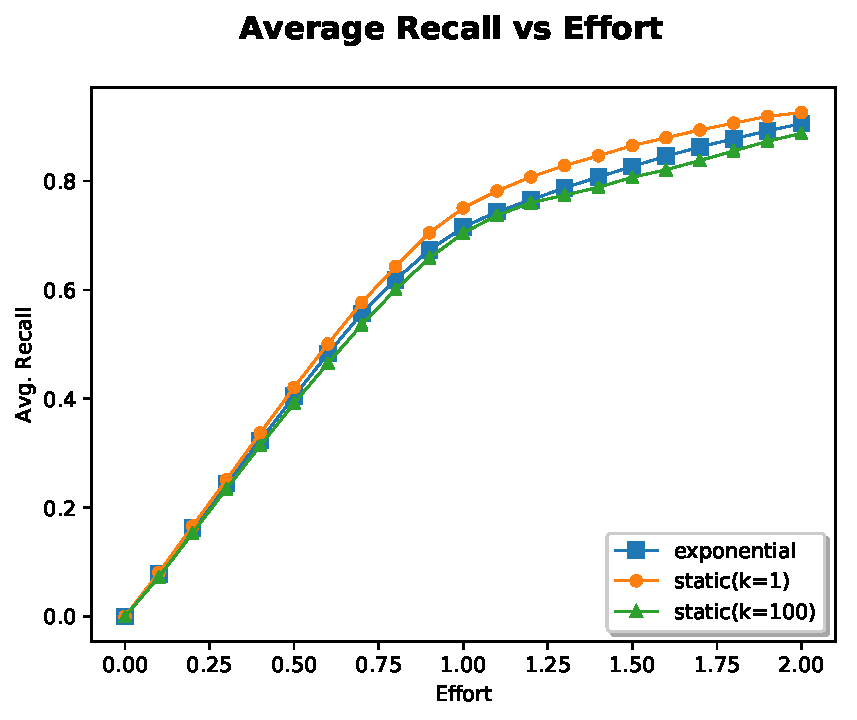
\includegraphics[width=\textwidth]{plots/bmi_static.pdf}
        \caption{Comparison of \texttt{bmi} and \texttt{static}.
            \texttt{static(k=1)} consistently outperforms the rest.}
        \label{plot:bmi_static}
    \end{subfigure}
    ~
    \begin{subfigure}[t]{0.48\textwidth}
        \centering
        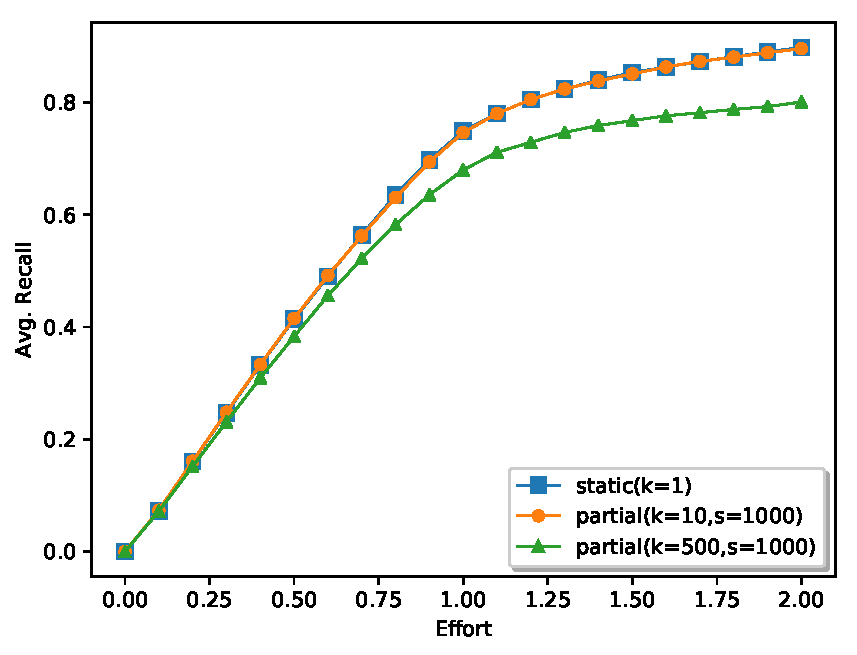
\includegraphics[width=\textwidth]{plots/static_partial.pdf}
        \caption{Comparison of \texttt{partial} and \texttt{static(k=1)}. We fix
            the partial set size to 1000 and observe that
            \texttt{partial(k=100,s=1000)} performs very similar to
        \texttt{static(k=1)}.}
        \label{plot:partial1}
    \end{subfigure}

    \begin{subfigure}[t]{0.48\textwidth}
        \centering
        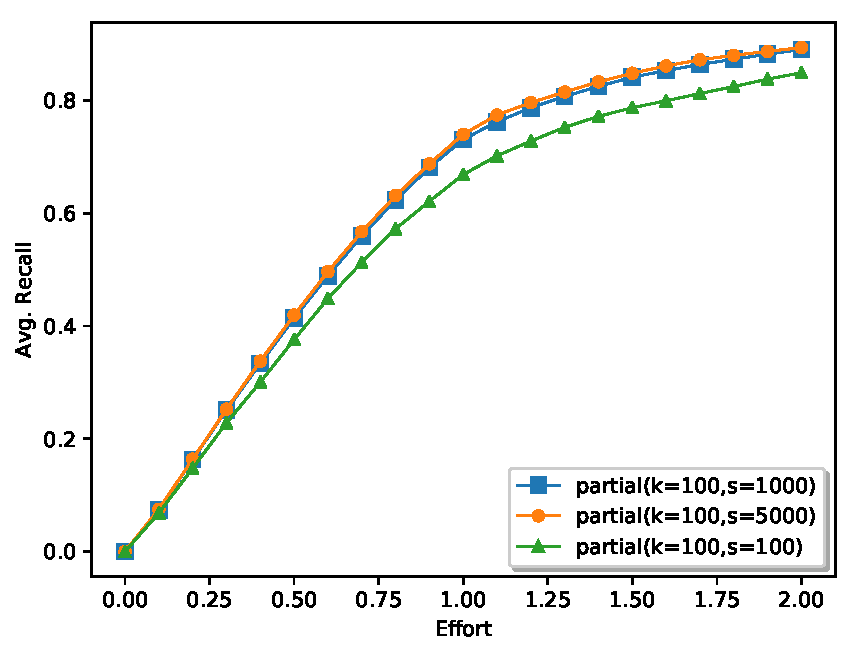
\includegraphics[width=\textwidth]{plots/partial2.pdf}
        \caption{Effect of partial set size on effectiveness. We observe that
        increasing the partial set size beyond 1000 doesn't have any benefit.}
        \label{plot:partial2}
    \end{subfigure}
    ~
    \begin{subfigure}[t]{0.48\textwidth}
        \centering
        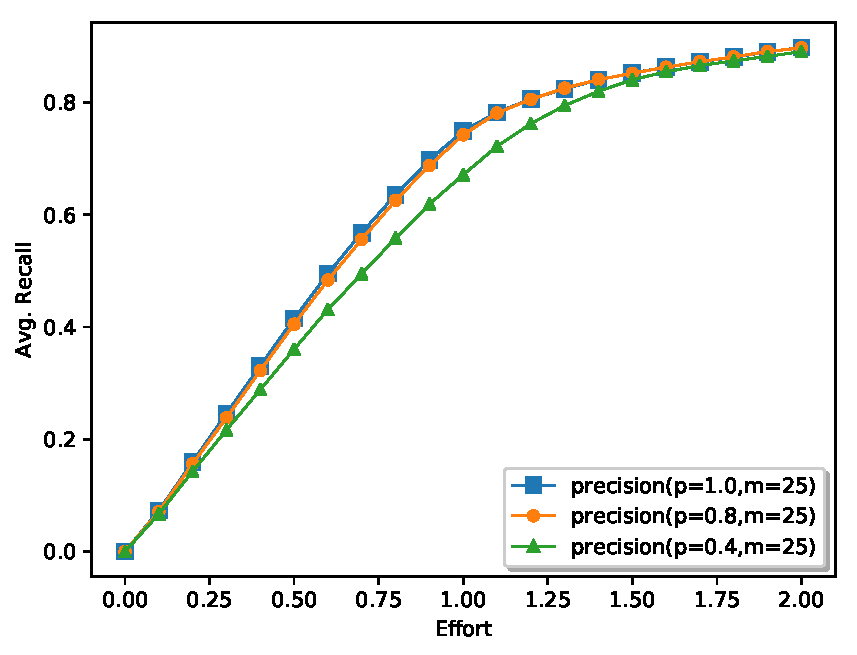
\includegraphics[width=\textwidth]{plots/precision.pdf}
        \caption{Comparison of various settings in \texttt{precision}.}
        \label{plot:prec}
    \end{subfigure}
    \caption{Comparison of various refresh strategies}
\end{figure}


\subsection*{Precision Based Refreshing}

Figure~\ref{plot:prec} compares the gain curves for
various settings of \texttt{precision}.

In this strategy, we fixed \texttt{m=25} and varied \texttt{p}. For
\texttt{p=0.8} and \texttt{p=1.0}, \texttt{precision} achieves $75\%$ recall at
$E_{norm} = 1$ which is similar to \texttt{static(k=1)}. This
similarity of recall is also seen at $E_{norm} = 1.5$ and $E_{norm} = 2$. For
\texttt{precision(p=1.0)}, CAL refreshes whenever a non-relevant judgment
is made, thus behaving very similar to \texttt{static(k=1)}. For
smaller values of \texttt{p}, we observe lower recall values during the initial stages; 
$73.5\%$ and $69.8\%$ recall at $E_{norm} = 1$ for \texttt{precision(p=0.6)} and
\texttt{precision(p=0.4)}, respectively. However, they catch up to
\texttt{static(k=1)} at higher $E_{norm}$, as relevant documents
become rarer; $85.9\%$ and $84.9\%$ recall at $E_{norm} = 1.5$ for
\texttt{precision(p=0.6)} and \texttt{precision(p=0.4)}, respectively.

This strategy improved the running time of simulations by $15\%$
on average when compared to \texttt{static(k=1)}.
\texttt{precision} strategies triggers lower number of refreshes during the
beginning of the CAL process when relevant documents are easier to find. During
the later stages when the relevant documents are harder to find,
\texttt{precision} strategies tend to keep refreshing after every judgment.
Figure~\ref{plot:prec2} compares the \texttt{precision} strategies with
\texttt{static(k=1)} based on how many refreshes were performed to achieve a
certain recall. The \texttt{precision} strategies find a lot of relevant
documents initially since they are easy to find and the precision of CAL's
output is high. \texttt{static(k=1)} keeps refreshing steadily irrespective of
the output quality. As relevant documents become harder to find, we find that
the \texttt{precision} strategies start refreshing as frequently as
\texttt{static(k=1)}.

\begin{figure}
    \centering
    \includegraphics[width=0.6\textwidth]{plots/prec2.pdf}
    \caption{Number of refreshes required to achieve a certain recall.}
    \label{plot:prec2}
\end{figure}


\subsection*{Effect of Training Iterations}

In all the previously discussed strategies, the improvement in running time over
\texttt{static(k=1)} is either due to refreshing less often (\texttt{bmi},
\texttt{precision}) or by optimizing scoring during a refresh
(\texttt{partial}). The running time of scoring can be further improved by just
increasing the number of threads. However, training is another expensive step
which cannot be trivially distributed across multiple threads. One way to
significantly reduce the training time is by simply reducing the number of
training iterations (\texttt{it}). In our experiments, the average time to train a classifier
for 100000 (default), 10000, and 1000 number of iterations was 265ms, 33ms, and
4ms respectively.

Despite these massive improvements in the running time, reducing the number of
iterations \texttt{it} beyond a certain point will directly
reduces the quality of the classifier, and thus harming the effectiveness of
CAL. Figure~\ref{plot:train} shows the impact of \texttt{it} on the gain curves
of \texttt{static(k=1)}. We find that reducing \texttt{it} from 100000 to 10000
didn't do any noticeable affect on the recalls. This suggests that setting
\texttt{it=10000} for all our experiments on \texttt{athome1} might have been
enough for the classifier to converge. Beyond this, we observe noticeable loss in
performance.

\begin{figure}
    \centering
    \begin{subfigure}[b]{0.48\textwidth}
        \centering
        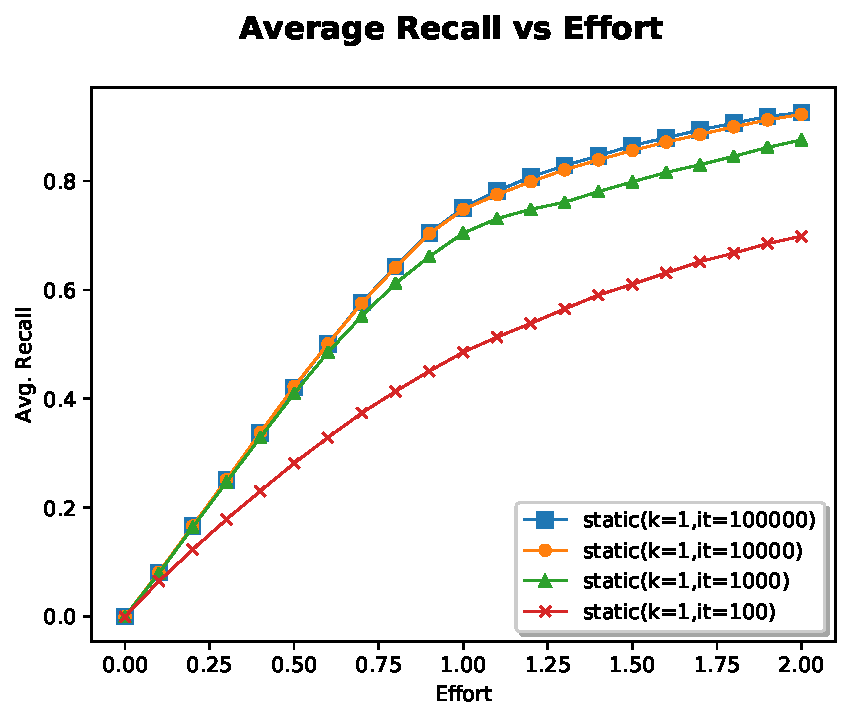
\includegraphics[width=\textwidth]{plots/training.pdf}
        \caption{Effect of number of training iterations on recall}
        \label{plot:train}
    \end{subfigure}
    ~
    \begin{subfigure}[b]{0.48\textwidth}
        \centering
        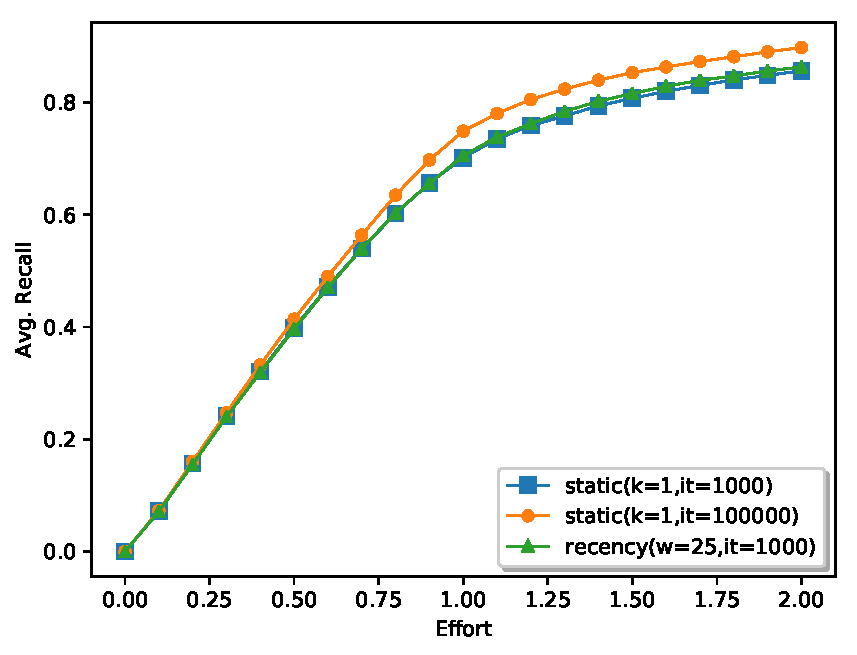
\includegraphics[width=\textwidth]{plots/recency.pdf}
        \caption{Effect of recency weighting on settings with low number of
        training iterations}
        \label{plot:recency}
    \end{subfigure}
    \caption{Gain curves comparing the effect of training iterations and recency
    weighting}
\end{figure}

\subsection*{Recency Weighting}

During our initial experiments, recency weighting seemed to have no
impact on the recall values. By reducing the number of training iterations
to $1000$, we introduced significant degradation in the system's effectiveness.
Reducing the number of training iterations also
reduced the running time of simulation by $76\%$ when compared to
\texttt{static(k=1)}. We used recency weighting to see whether it could recover
the lost effectiveness.  \texttt{recency(w=1,it=1000)} is equivalent to
\texttt{static(k=1,it=1000)} and it achieves $70.4\%$ and $79.8\%$
recall when $E_{norm}$ is equal to $1$ and $1.5$ respectively. By increasing
$w$, we observe an increase in recall for $E_{norm} \in \{1.5, 2\}$. However,
the recall is consistently and significantly lower when compared to
\texttt{static(k=1,it=100000)}. For example, \texttt{recency(w=10,it=1000)} is
only able to achieve $82.4\%$ recall at $E_{norm}=1.5$, while
\texttt{static(k=1,it=100000)} achieves $86.5\%$ recall at the same effort.


\begin{table*}[]
\centering
\caption{Summary of results for recency weighting}
\label{table.recency}
\resizebox{\textwidth}{!}{%
\begin{tabular}{|c|c|c|c|c|c|}
\hline
\textbf{Strategy} & \begin{tabular}[x]{@{}c@{}}
    \textbf{Avg. Recall}\\ \textbf{@($E_{norm}$=1)}
\end{tabular} & \begin{tabular}[x]{@{}c@{}}
\textbf{Avg. Recall}\\ \textbf{@($E_{norm}$=1.5)}
\end{tabular} & \begin{tabular}[x]{@{}c@{}}
\textbf{Avg. Recall}\\ \textbf{@($E_{norm}$=2)}
\end{tabular} & \begin{tabular}[x]{@{}c@{}}
\textbf{$E_{norm}$ for}\\ \textbf{75\% recall}
\end{tabular}&
\begin{tabular}[x]{@{}c@{}}
    \textbf{Running Time}\\ \textbf{(in min)}
\end{tabular} \\ \hline \hline
\texttt{recency(w=1,it=1000)} &  0.704 & 0.798 & 0.875 & 1.243 & 11.75 \\ \hline
\texttt{recency(w=2,it=1000)} &  0.705 & 0.806 & 0.884 & 1.219 & 11.66 \\ \hline
\texttt{recency(w=5,it=1000)} &  0.704 & 0.814 & 0.887 & 1.191 & 11.63\\ \hline
\texttt{recency(w=10,it=1000)} &  0.707 & 0.824 & 0.891 & 1.206 & 11.54\\ \hline
\end{tabular}
}
\end{table*}

% \begin{figure}
%  \centering 
%  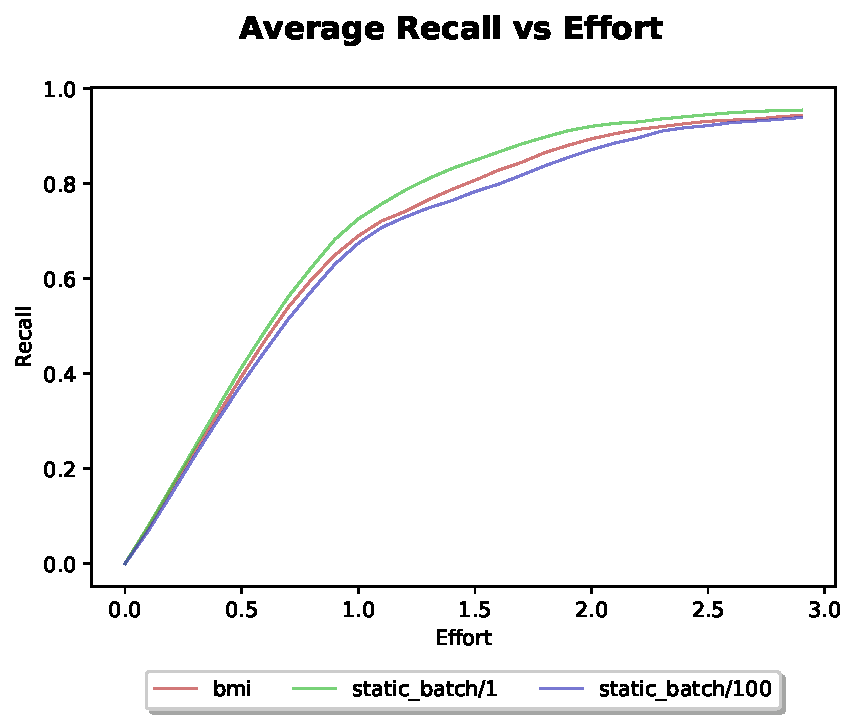
\includegraphics[width=1.0\linewidth]{static1.pdf}
%  \caption{Static Refresh}
%  \label{fig.static1}
% \end{figure}

% \begin{figure}
%  \centering 
%  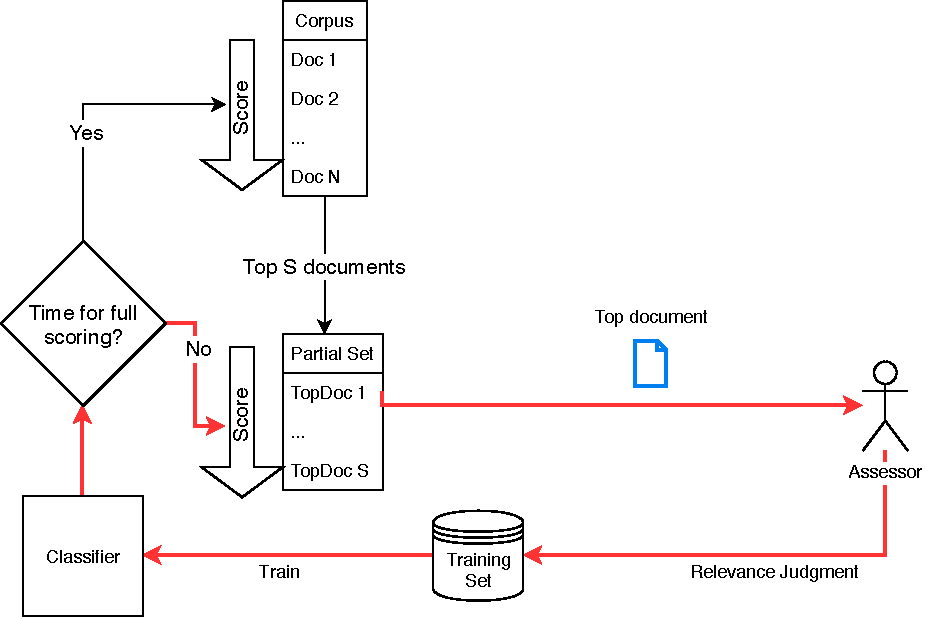
\includegraphics[width=1.0\linewidth]{partial1.pdf}
%  \caption{Partial Refresh}
%  \label{fig.partial1}
% \end{figure}

% \begin{figure}
%  \centering 
%  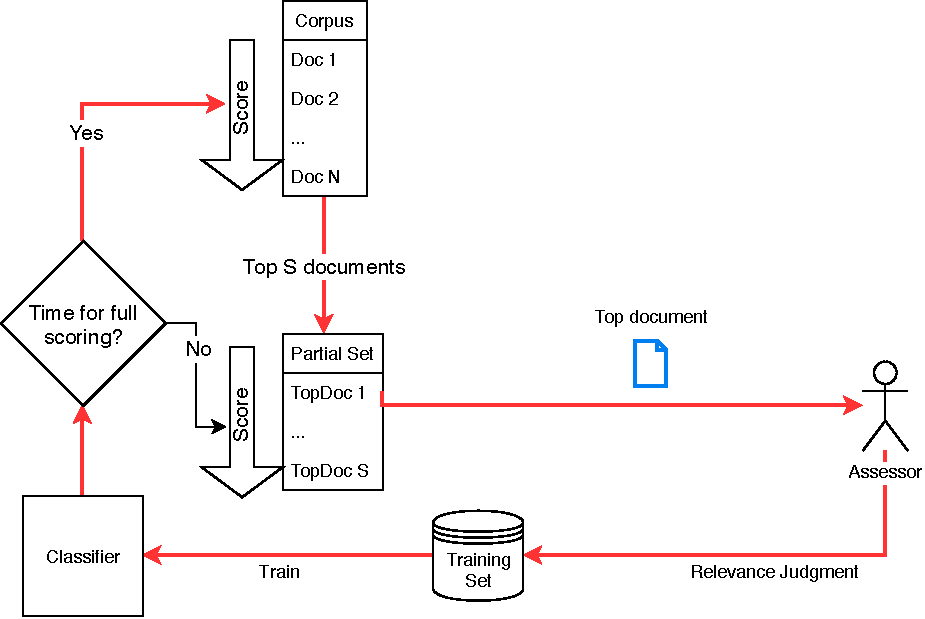
\includegraphics[width=1.0\linewidth]{partial2.pdf}
%  \caption{Partial Refresh}
%  \label{fig.partial2}
% \end{figure}

% \begin{figure}
%  \centering 
%  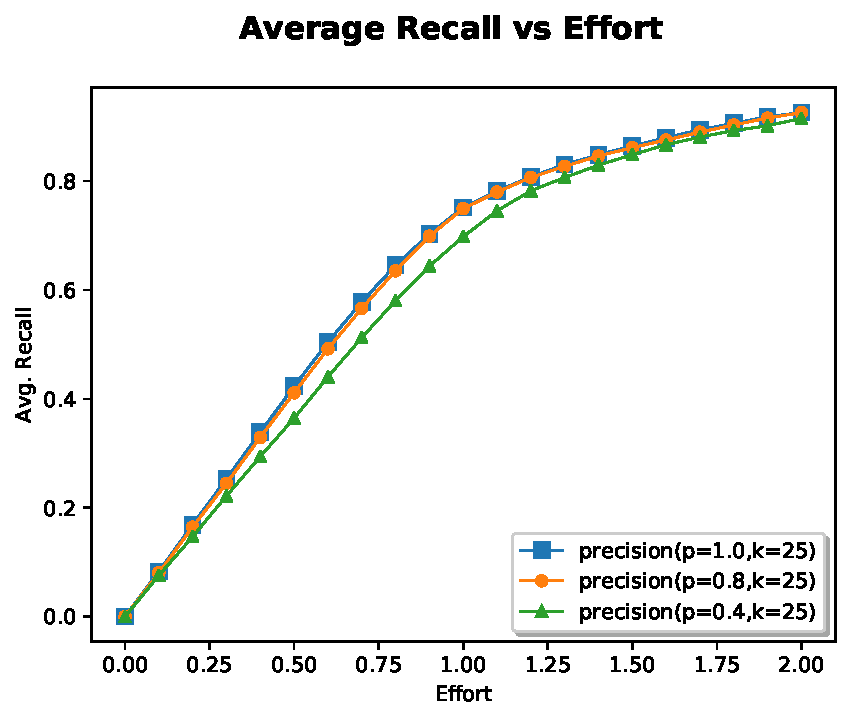
\includegraphics[width=1.0\linewidth]{prec1.pdf}
%  \caption{Precision Based Refresh}
%  \label{fig.prec1}
% \end{figure}

% \begin{figure}
%  \centering 
%  \includegraphics[width=1.0\linewidth]{prec2.pdf}
%  \caption{Precision Based Refresh}
%  \label{fig.prec2}
% \end{figure}

% \begin{figure}
%  \centering 
%  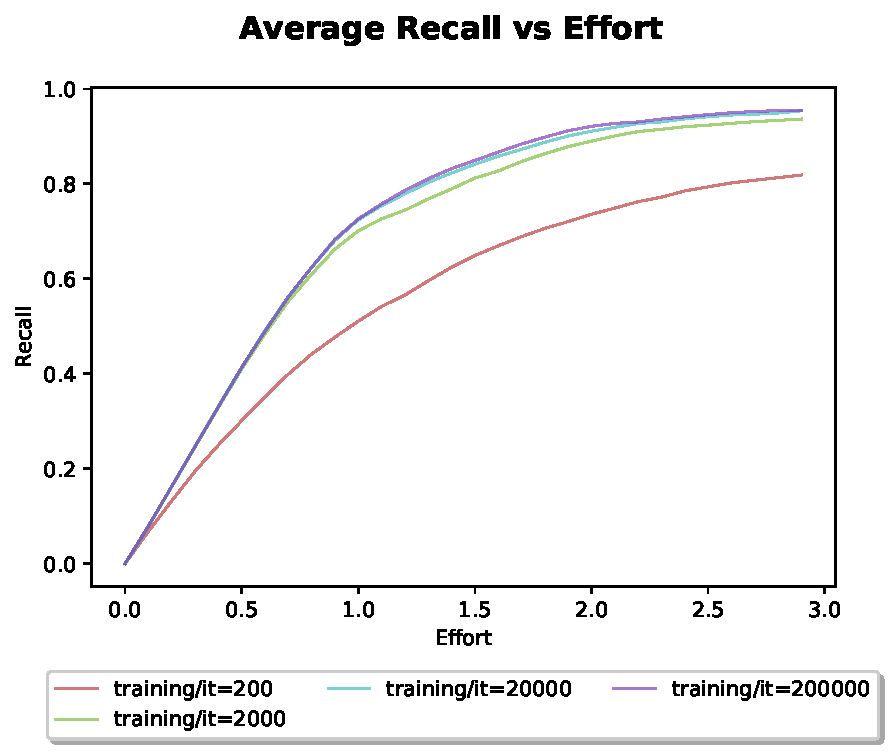
\includegraphics[width=1.0\linewidth]{train1.pdf}
%  \caption{Effect of number of training iterations}
%  \label{fig.train1}
% \end{figure}

% \begin{figure}
%  \centering 
%  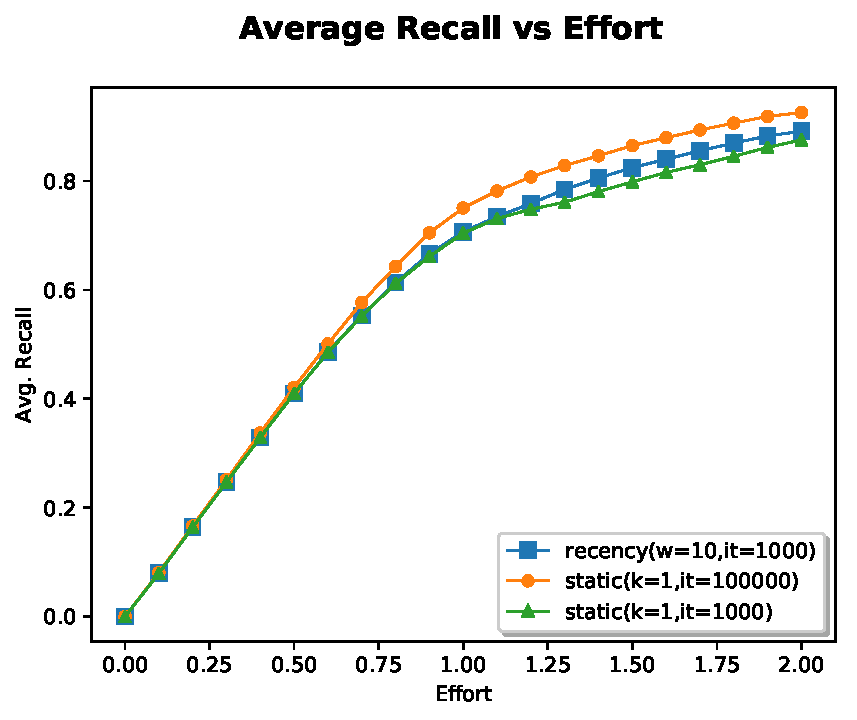
\includegraphics[width=1.0\linewidth]{rec1.pdf}
%  \caption{Recency Weighting}
%  \label{fig.recency1}
% \end{figure}
